\documentclass[a4j]{jsbook}
\usepackage[utf8]{inputenc}
\usepackage[dvipdfmx]{graphicx}
\usepackage{amsmath,ascmac, amssymb}
\usepackage{bm}
\usepackage{algorithm,algorithmic}
\usepackage{listings}
\usepackage{cases}
\usepackage{amsthm}
\usepackage{siunitx}
\usepackage{color}
\lstset{
  basicstyle={\ttfamily},
  identifierstyle={\small},
  commentstyle={\smallitshape},
  keywordstyle={\small\bfseries},
  ndkeywordstyle={\small},
  stringstyle={\small\ttfamily},
  frame={tb},
  breaklines=true,
  columns=[l]{fullflexible},
  numbers=left,
  xrightmargin=0zw,
  xleftmargin=3zw,
  numberstyle={\scriptsize},
  stepnumber=1,
  numbersep=1zw,
  lineskip=-0.5ex
}
\newtheorem{theorem}{定理}
\newtheorem{prop}[theorem]{命題}
\newtheorem{lemma}[theorem]{補題}
\newtheorem{cor}[theorem]{系}
\newtheorem{example}[theorem]{例}
\newtheorem{definition}[theorem]{定義}
\newtheorem{rem}[theorem]{注意}
\newtheorem{guide}[theorem]{参考}
\newtheorem{formula}[theorem]{公式}
\numberwithin{theorem}{chapter}  % 定理番号を「定理2.3」のように印刷

\title{「工業数学A3」講義ノート}
\author{担当教員: 矢ヶ崎 一幸}
\date{曜時限: 水曜1限}

\begin{document}

\maketitle

\tableofcontents

\newpage

\section*{講義概要}
本講義ではフーリエ解析と,それに関連の深いラプラス変換に関して,理論と応用について述べる.2回の小テストと期末試験により,成績評価を行う.具体的な割合としては,小テストが1回10点分,期末試験が80点分である.教科書として中村周『フーリエ解析』(朝倉書店)を用いるが,誤植が非常に多く,また本質的な間違いをしている部分もあるため,基本的にはこの講義ノートを参考にするとよい.なお,具体的な誤植については,PandAにアップロードした正誤表を確認すること.

\chapter{フーリエ級数展開}
\section{導入: 周期関数のフーリエ級数展開}
\(\mathbb{R}\)上の関数\(f(t)(t\in\mathbb{R})\)に対して,\(f\)が周期\(T\)の周期関数であるとは,
\begin{equation*}
    \forall t\in\mathbb{R}, f(t+T)=f(t)
\end{equation*}
となることを言う.このとき,\(\forall n\in\mathbb{Z}, f(t+nT)=f(t)(t\in\mathbb{R})\)も成立する.\\
 広いクラスの,周期\(T\)の周期関数に対して,\(f\)の\textcolor{red}{フーリエ級数展開}は
\begin{equation}
    f(t)=c+\sum_{n=1}^\infty a[n]\cos n\omega t+\sum_{n=1}^\infty b[n]\sin n\omega t \label{eq1-1}
\end{equation}
と定義される.但し,\(\displaystyle \omega=\frac{2\pi}{T}, c, a[n], b[n]\)は定数である.\eqref{eq1-1}の右辺の級数が「収束」すればフーリエ級数展開が定義できるが,本講義では,\eqref{eq1-1}がどのようなときに成り立ち,そのときどのような意味で収束するのかについて述べる.
\section{三角関数の直交関係とフーリエ係数}
\eqref{eq1-1}において,\(a[n], b[n](n=1, 2, \dots)\)のことを\textcolor{red}{フーリエ係数}という.この計算には,次の定理を用いる.
\begin{theorem}\upshape{\bf{(三角関数の直交関係)}}
\label{th1-1}
\begin{equation}
    \frac{2}{T}\int_0^T \cos n\omega t\cos m\omega t\mathrm{d}t=\delta_{nm} \label{eq1-2}
\end{equation}
\begin{equation}
    \frac{2}{T}\int_0^T \sin n\omega t\sin m\omega t\mathrm{d}t=\delta_{nm} \label{eq1-3}
\end{equation}
\begin{equation}
    \frac{2}{T}\int_0^T \sin n\omega t\cos m\omega t\mathrm{d}t=0 \label{eq1-4}
\end{equation}
\begin{equation}
    \frac{2}{T}\int_0^T \cos n\omega t\mathrm{d}t=\frac{2}{T}\int_0^T \sin n\omega t=0 \label{eq1-5}
\end{equation}
が成り立つ.ここで,\(\delta_{nm}\)は\textcolor{red}{クロネッカーのデルタ}である.
\end{theorem}
\begin{proof}
三角関数の積和の公式から
\begin{equation*}
    \cos n\omega t\cos m\omega t=\frac{1}{2}\left(\cos\omega(n+m)t+\cos\omega(n-m)t\right)
\end{equation*}
となる.一方,任意の0でない整数\(k\)に対して
\begin{equation*}
    \frac{1}{T}\int_0^T\cos k\omega t\mathrm{d}t=\left[\frac{\sin\omega kt}{2\pi k}\right]_0^T=0
\end{equation*}
なので
\begin{equation*}
    \frac{2}{T}\int_0^T \cos n\omega t\cos m\omega t\mathrm{d}t=\frac{1}{T}\int_0^T \cos\omega(n-m)t\mathrm{d}t
\end{equation*}
この右辺は,\(n\neq m\)のときは上式より0になる.\(n=m\)のときは,定数1の積分だから右辺は1になる.よって\eqref{eq1-2}が示された.他の式についても同様に示せる.
\end{proof}
積分と無限級数の和の順序交換ができる
\footnote{
正確には,
\begin{equation*}
    \sum_{n=1}^\infty\int_a^b g_n(x)\mathrm{d}x=\int_a^b\sum_{n=1}^\infty g_n(x)\mathrm{d}x
\end{equation*}
が成立するためには,\(g_n(x)\)がある関数に一様収束することが必要である.
}
と仮定して,フーリエ級数展開の式からフーリエ係数を求める.まず,\eqref{eq1-1}を0から\(T\)まで積分すると,\eqref{eq1-5}より
\begin{equation*}
    \frac{1}{T}\int_0^T f(t)\mathrm{d}t=\frac{1}{T}\int_0^T c\mathrm{d}t=c
\end{equation*}
となる.また,\(\cos\omega mt\)をかけて積分すると,\eqref{eq1-2},\eqref{eq1-4},\eqref{eq1-5}を用いて
\begin{eqnarray*}
\frac{2}{T}\int_0^T f(t)\cos m\omega t\mathrm{d}t&=&\sum_{n=1}^\infty\frac{2}{T}\int_0^T a[n]\cos n\omega t\cos m\omega t\mathrm{d}t \\
&=&\sum_{n=1}^\infty a[n]\delta_{nm}=a[m]
\end{eqnarray*}
となる.同様に,\eqref{eq1-3},\eqref{eq1-4},\eqref{eq1-5}を用いて
\begin{equation*}
    \frac{2}{T}\int_0^T f(t)\sin m\omega t\mathrm{d}t=\sum_{n=1}^\infty b[n]\delta_{nm}=b[m]
\end{equation*}
が得られる.記号を簡単にするために\(a[0]=2c\)と書くことにすれば,以上の計算から次の公式が得られる.
\begin{formula}
\label{formula1-2}
\begin{equation}
    f(t)=\frac{a[0]}{2}+\sum_{n=1}^\infty a[n]\cos n\omega t+\sum_{n=1}^\infty b[n]\sin n\omega t \label{eq1-6}
\end{equation}
ならば,
\begin{eqnarray}
a[n]&=&\frac{2}{T}\int_0^T f(t)\cos n\omega t\mathrm{d}t (n=0, 1, 2, \dots) \\
b[n]&=&\frac{2}{T}\int_0^T f(t)\sin n\omega t\mathrm{d}t (n=1, 2, \dots)
\end{eqnarray}
である.
\end{formula}
周期性により,
\begin{eqnarray}
a[n]&=&\frac{2}{T}\int_{-\frac{T}{2}}^{\frac{T}{2}} f(t)\cos n\omega t\mathrm{d}t (n=0, 1, 2, \dots) \\
b[n]&=&\frac{2}{T}\int_{-\frac{T}{2}}^{\frac{T}{2}} f(t)\sin n\omega t\mathrm{d}t (n=1, 2, \dots)
\end{eqnarray}
が成立する.\(f\)が偶関数ならば,\(b[n]=0(n=1, 2, \ldots)\)であり,
\begin{equation*}
    f(t)=\frac{a[0]}{2}+\sum_{n=1}^\infty a[n]\cos n\omega t
\end{equation*}
となる.これを\textcolor{red}{余弦フーリエ級数展開}という.また,\(f\)が奇関数ならば,\(a[n]=0(n=0, 1, 2, \ldots)\)であり,
\begin{equation*}
    f(t)=\frac{a[0]}{2}+\sum_{n=1}^\infty b[n]\sin n\omega t
\end{equation*}
となる.これを\textcolor{red}{正弦フーリエ級数展開}という.
\section{複素フーリエ変換}
オイラーの公式\(e^{i\theta}=\cos\theta+i\sin\theta(i\mbox{は虚数単位})\)により,
\begin{equation*}
    \cos\theta=\frac{1}{2}\left(e^{i\theta}+e^{-i\theta}\right), \sin\theta=\frac{1}{2i}\left(e^{i\theta}-e^{-i\theta}\right)
\end{equation*}
が成立する.すると,フーリエ級数展開\eqref{eq1-6}は
\begin{equation*}
    f(t)=\frac{a[0]}{2}+\sum_{n=1}^\infty\left(\frac{a[n]}{2}+\frac{b[n]}{2i}\right)e^{in\omega t}+\sum_{n=1}^\infty\left(\frac{a[n]}{2}-\frac{b[n]}{2i}\right)e^{-in\omega t}
\end{equation*}
のように表される.
\begin{equation*}
    c[n]=\begin{cases}
    \frac{a[0]}{2} & (n=0) \\
    \frac{a[n]-ib[n]}{2} & (n>0) \\
    \frac{a[-n]+ib[-n]}{2} & (n<0)
    \end{cases}
\end{equation*}
とすると,\textcolor{red}{複素フーリエ級数展開}
\begin{equation}
    f(t)=\sum_{n=-\infty}^\infty c[n]e^{in\omega t}
\end{equation}
が定義できる.公式1.2or直接計算することにより
\begin{equation*}
    c[n]=\frac{1}{T}\int_0^T f(t)e^{-in\omega t}\mathrm{d}t (n\in\mathbb{Z})
\end{equation*}
が得られる.
\section{いくつかの実例}
\begin{example}\upshape{\bf{(三角多項式)}} 
\label{ex1-1}
三角多項式とは,\(\sin\omega t, \cos\omega t\)の多項式である.例えば,
\begin{equation*}
    f_1(t)=(\cos\omega t)^3=\frac{3}{4}\cos\omega t+\frac{1}{4}\cos 3\omega t
\end{equation*}
は三角多項式である.一般に,ある\(N\in\mathbb{N}\)が存在して,
\begin{equation*}
    f(t)=\sum_{n=-N}^N c[n]e^{in\omega t}
\end{equation*}
と表されるとき,\(f(t)\)は三角多項式となる.
\end{example}
\begin{example}\upshape{\bf{(三角波)}} 
\label{ex1-2}
\(f_2(t)\)を\(\displaystyle |t|\leq\frac{T}{2}\)では
\begin{equation*}
    f_2(t)=|t|
\end{equation*}
それ以外では周期的に拡張された周期\(T\)の連続な周期関数とする.\(f_2(t)\)は偶関数であるから,余弦フーリエ級数展開を持ち,
\begin{equation*}
    a[n]=\frac{2}{T}\int_{-\frac{T}{2}}^{\frac{T}{2}}|t|\cos n\omega t\mathrm{d}t=\frac{4}{T}\int_0^{\frac{T}{2}} t\cos n\omega t\mathrm{d}t
\end{equation*}
となる.\(n=0\)のとき
\begin{equation*}
    a[0]=\frac{4}{T}\left[\frac{t^2}{2}\right]_0^{\frac{T}{2}}=\frac{T}{2}
\end{equation*}
であり,\(n\neq 0\)のとき
\begin{equation*}
    a[n]= \begin{cases}
    0 & (n: \mbox{偶数}) \\
    -\frac{4}{\pi n^2\omega} & (n: \mbox{奇数})
    \end{cases}
\end{equation*}
である.
\end{example}
\begin{example}
\label{ex1-3}
\begin{equation*}
    f_3(t)=\frac{1}{\frac{5}{4}+\cos\omega t}
\end{equation*}
留数定理を用いると\(f_3(t)\)のフーリエ級数を計算出来て,\(n\geq 0\)のとき
\begin{equation*}
    c[-n]=\frac{4}{3}(-2)^{-n}
\end{equation*}
となる.また,\(n>0\)のときは\(c[n]=c[-n]\)より\(\displaystyle c[n]=\frac{4}{3}(-2)^{-n}\)となるから
\begin{equation*}
    f_3(t)=\frac{4}{3}+\sum_{n=1}^\infty \frac{4}{3}(-2)^{-n}\left(e^{in\omega t}+e^{-in\omega t}\right)
\end{equation*}
となる.
\end{example}
\section{フーリエ級数の一様収束}
前節の例から想像されるように,広いクラスの周期関数\(f(t)\)に対してフーリエ級数展開が定義されるが,奇妙な例を考えると,連続でありながらフーリエ級数が収束しない点を持つ場合がある.このような,フーリエ級数の収束の問題は,数学的には興味深い問題だが,ここでは深入りせず,一つだけ定理を紹介するにとどめる.\\
 \(\mathbb{R}\)上の関数\(f(t)\)が\textcolor{red}{リプシッツ連続}であるとは
\begin{equation*}
    \exists C>0 \ \mathrm{s.t.} \ \forall t, s\in\mathbb{R} \ |f(t)-f(s)|\leq C|t-s|
\end{equation*}
となることをいう.
\begin{theorem}
\label{th1-3}
\(f(t)\)がリプシッツ連続な周期関数ならば,フーリエ級数展開は\(f(t)\)に一様に収束する.
\end{theorem}
この定理を証明することが本章の目標となる.
\section{有限フーリエ級数}
フーリエ級数の理論の美しい点の一つは,幾何学的な構造を持つことである.すなわち,フーリエ級数展開とは,「関数のなす線形空間」のベクトルの,基底による直交分解であると考えることができる.この考え方を完全に述べるには関数解析の理論(ヒルベルト空間論)の知識が必要となるため,ここでは述べない.以下では主要なアイデアのみ述べる.\\
 最初に線形代数の復習をしておこう.\(X=\mathbb{C}^N\)を\(N\)次元複素線形空間とする.また,その元を\(u=(u[0], \cdots, u[N-1])\in X\)とする.\(u, v\in X\)のエルミート内積は
\begin{equation*}
    \langle u, v\rangle=\sum_{n=0}^{N-1} u[n]\overline{v[n]}
\end{equation*}
で定義される.また,\(|u|=\sqrt{\langle u, u\rangle}\)は\(u\in X\)の長さである.\(u_0, \cdots, u_{M-1}\in X\)が正規直交系であるとは
\begin{equation*}
    \langle u_n, u_m\rangle=\delta_{nm} (n, m=0, \dots, M-1)
\end{equation*}
となることをいう.\(N=M\)のときこれらは正規直交基底と呼ばれ,
\begin{equation*}
    \forall u\in X, u=\sum_{n=0}^{N-1}\langle u, u_n\rangle u_n
\end{equation*}
が成立する.ここで,\(\langle u, u_n\rangle\)を座標成分という.\(\mathbb{C}^N\)の標準的な基底\(\bm{e}_n[k]=\delta_{kn}(n, k=0, \dots, N-1)\)は正規直交基底となる.\\
 \(\displaystyle\alpha=\frac{2\pi}{N}\)として,
\begin{equation*}
    \varphi_n[k]=\frac{1}{\sqrt{N}}\exp(i\alpha nk) (n, k=0, \dots, N-1)
\end{equation*}
を考える.
\begin{prop}
\label{prop1-4}
\(\{\varphi_0, \dots, \varphi_{N-1}\}\)は\(X(=\mathbb{C}^N)\)の正規直交基底となる.
\end{prop}
\begin{proof}
最初に
\begin{equation*}
    |\varphi_n|^2=\langle\varphi_n, \varphi_n\rangle=\frac{1}{N}\sum_{k=0}^{N-1}\left|e^{i\alpha nk}\right|^2=1
\end{equation*}
だから,各\(\varphi_n\)のノルムは1である.\(n\neq m\)のときは
\begin{eqnarray*}
\langle\varphi_n, \varphi_m\rangle&=&\frac{1}{N}\sum_{k=0}^{N-1}e^{i\alpha nk}e^{-i\alpha mk} \\
&=&\frac{1}{N}\cdot\frac{1-e^{i\alpha(n-m)N}}{1-e^{i\alpha(n-m)}}=0
\end{eqnarray*}
となる.ここで,等比級数の和の公式と,\(\alpha N=2\pi\)を用いた.
\end{proof}
\(u\in X\)とする.
\begin{equation}
    \hat{u}[n]=\langle u, \varphi_n\rangle=\frac{1}{\sqrt{N}}\sum_{k=0}^{N-1}u[k]e^{-i\alpha nk} (n=0, \dots, N-1) \label{eq1-12}
\end{equation}
とおくと,
\begin{equation}
    u[k]=\sum_{n=0}^{N-1}\hat{u}[n]\varphi_n[k]=\frac{1}{\sqrt{N}}\sum_{n=0}^{N-1}\hat{u}[n]e^{i\alpha nk} (k=0, \dots, N-1) \label{eq1-13}
\end{equation}
と書ける.\eqref{eq1-12}を\textcolor{red}{有限フーリエ変換},\eqref{eq1-13}を\textcolor{red}{逆有限フーリエ変換},または\(\hat{u}[n]\)の\textcolor{red}{有限フーリエ級数展開}と呼ぶ.\\
 有限フーリエ変換,逆有限フーリエ変換はユニタリーな線形変換である.つまり
\begin{equation}
    |u|=|\hat{u}| \label{eq1-14}
\end{equation}
が成立する.
\begin{proof}
\(u, v\in X\)のとき,\(u, v\)の内積にそれぞれの有限フーリエ級数展開を代入すると
\begin{eqnarray*}
\langle u, v\rangle&=&\sum_{n=0}^{N-1}\sum_{m=0}^{N-1}\langle \hat{u}[n]\varphi_n, \hat{v}[m]\varphi_m\rangle \\
&=&\sum_{n=0}^{N-1}\sum_{m=0}^{N-1}\hat{u}[n]\overline{\hat{v}[m]}\delta_{nm} \\
&=&\sum_{n=0}^{N-1}\hat{u}[n]\overline{\hat{v}[n]}=\langle\hat{u}, \hat{v}\rangle
\end{eqnarray*}
となる.すなわち
\begin{equation}
    \langle u, v\rangle=\langle\hat{u}, \hat{v}\rangle \label{eq1-15}
\end{equation}
が示された.
\end{proof}
\section{有限フーリエ級数の連続極限}
さて,有限フーリエ級数の極限として元の関数が得られることを証明しておこう.
\begin{theorem}
\label{th1-5}
\(f(t)\)を周期\(T\)のリプシッツ連続な周期関数とする.\(\displaystyle\omega=\frac{2\pi}{T}, \alpha=\frac{2\pi}{N}\)として,
\begin{equation*}
    f_N(t)=\sum_{-\frac{N}{2}\leq n<\frac{N}{2}} c_N[n]e^{in\omega t}
\end{equation*}
\begin{equation*}
    c_N[n]=\frac{1}{N}\sum_{m=0}^{N-1}f\left(\frac{m}{N}T\right)e^{-i\alpha nm} (n\in\mathbb{Z})
\end{equation*}
とする.このとき,\(f_N(t)\)は\(f(t)\)に一様収束する.
\end{theorem}
\begin{rem}
\label{rem1-1}
\begin{equation*}
    f_N\left(\frac{k}{N}T\right)=\sum_{-\frac{N}{2}\leq n<\frac{N}{2}}c_N[n]e^{i\alpha nk}=\sum_{n=0}^{N-1}c_N[n]e^{i\alpha nk}=f\left(\frac{k}{N}T\right)
\end{equation*}
が成立する.つまり,\(f_N(t)\)は\(\displaystyle f(t_k)\left(t_k:=\frac{k}{N}T\right)\)の値を与えた時の補間多項式となっている.
\end{rem}
\begin{proof}
まず
\begin{equation*}
    d_N[n]=\frac{1}{N}\sum_{m=0}^{N-1}\left(f\left(\frac{m}{N}T\right)-f\left(\frac{m-1}{N}T\right)\right)e^{-2\pi i\frac{m}{N}n}
\end{equation*}
とおく.\(\{d_N[n]\}\)は\(\displaystyle f(t_n)-f\left(t_n-\frac{T}{N}\right)\)の有限フーリエ変換の\(\displaystyle\frac{1}{\sqrt{N}}\)倍である.リプシッツ連続性の仮定より,ある\(L>0\)が存在して
\begin{equation*}
    \left|f\left(\frac{m}{N}T\right)-f\left(\frac{m-1}{N}T\right)\right|\leq L\frac{T}{N} (m\in\mathbb{Z})
\end{equation*}
となる.\(C:=LT\)とおくと
\begin{equation*}
    \left|f\left(\frac{m}{N}T\right)-f\left(\frac{m-1}{N}T\right)\right|\leq \frac{C}{N} (m\in\mathbb{Z})
\end{equation*}
が成り立つ.従って,有限フーリエ変換の等長性\eqref{eq1-14}より
\begin{equation*}
    N\sum_{k=0}^{N-1}\left|d_N[k]\right|^2\leq\sum_{m=0}^{N-1}\left|\frac{C}{N}\right|^2=\frac{C^2}{N}
\end{equation*}
すなわち
\begin{equation*}
    \sum_{k=0}^{N-1}\left|d_N[k]\right|^2\leq\frac{C^2}{N^2}
\end{equation*}
が従う.一方,\(d_N[k]\)の定義より
\begin{equation*}
    d_N[k]=\left(1-e^{-2\pi i\frac{k}{N}}\right)c_N[k]=2ie^{-\pi i\frac{k}{N}}\sin\left(\frac{\pi k}{N}\right)c_N[k]
\end{equation*}
となる.従って
\begin{equation}
    |\sin\theta|\geq\frac{2}{\pi}|\theta| \left(|\theta|\leq\frac{\pi}{2}\right) \label{eq1-16}
\end{equation}
を用いれば
\begin{equation*}
    \left|d_N[k]\right|\geq\frac{4|k|}{N}\left|c_N[k]\right|
\end{equation*}
が従う.\(d_N[k]\)が周期\(N\)を持つことに注意して,これらを組み合わせると
\begin{equation*}
    \sum_{-\frac{N}{2}\leq k<\frac{N}{2}}|k|^2|c_N[k]|^2\leq\frac{C^2}{16}
\end{equation*}
が導かれる.そこで
\begin{equation*}
    f_N'(t)=\sum_{n}in\omega c_N[n]e^{in\omega t}
\end{equation*}
の絶対値を考えると,
\begin{eqnarray}
|f_N'(t)|&\leq&\omega\sqrt{N}\sum_{n}\frac{|n|}{\sqrt{N}}|c_N[n]| \nonumber \\
&\leq&\omega\sqrt{N}\left(\sum_{n}\left(\frac{1}{\sqrt{N}}\right)^2\right)^{\frac{1}{2}}\left(\sum_{n}|n|^2|c_N[n]|^2\right)^{\frac{1}{2}} \nonumber \\
&\leq&\sqrt{N}C' (C'\mbox{はある定数}) \label{eq1-17}
\end{eqnarray}
が得られる.ここで,第2の不等式ではシュワルツの不等式: \(|u\cdot v|\leq|u||v|\)を用いた.\\
 さて,任意の\(t\in[0, T]\)に対して,\(\displaystyle |t-t_k|\leq\frac{T}{2N}\)であるような\(\displaystyle t_k=\frac{k}{N}T\)が存在する.\(f(t_k)=f_N(t_k)\)に注意して
\begin{eqnarray*}
f(t)-f_N(t)&=&(f(t)-f(t_k))+(f(t_k)-f_N(t_k))+(f_N(t_k)-f_N(t)) \\
&=&(f(t)-f(t_k))+(f_N(t_k)-f_N(t))
\end{eqnarray*}
と分解して考える.\(f(t)\)のリプシッツ連続性と,\(f_N'\)の微分の評価\eqref{eq1-17}から
\begin{equation*}
    |f(t)-f_N(t)|\leq C|t-t_k|+C'\sqrt{N}|t-t_k|=O\left(\frac{1}{\sqrt{N}}\right)
\end{equation*}
が得られる.つまり,\(N\to\infty\)のとき\(f_N(t)\)が\(f(t)\)に一様収束することが示せた.
\end{proof}
\section{関数の空間の内積と直交関数系}
\(X\)を周期\(T\)の有界な周期関数で,\([0, T]\)上で積分可能な関数全体の集合とする.\(f, g\in X\)に対して,これらの\textcolor{red}{内積}を
\begin{equation*}
    \langle f, g\rangle=\frac{1}{T}\int_0^T f(t)\overline{g(t)}\mathrm{d}t
\end{equation*}
で定義する.この内積は次のような性質を満たす: \(f, g, h\in X, a, b\in\mathbb{C}\)とするとき
\begin{eqnarray*}
\langle af+bg, h\rangle&=&a\langle f, h\rangle+b\langle g, h\rangle \\
\langle f, g+bh\rangle&=&\Bar{a}\langle f, g\rangle+\Bar{b}\langle f, h\rangle \\
\langle f, g\rangle&=&\overline{\langle g, f\rangle}
\end{eqnarray*}
また,\(f\in X\)に対して
\begin{equation*}
    ||f||=\sqrt{\langle f, f\rangle}=\left(\frac{1}{T}\int_0^T |f(t)|^2\mathrm{d}t\right)^{\frac{1}{2}}\geq 0
\end{equation*}
を\(f\)の\textcolor{red}{ノルム}(または\(L^2\)-ノルム)という.\(||f||=0\)であれば,\(f\)は実質上(ほとんど至るところで
\footnote{
測度空間において,ある性質\(P\)を満たさない集合の測度が0である場合,ほとんど至るところで\(P\)を満たすという.
}
)0の関数である.\\
 次に,シュワルツの不等式と三角不等式を示しておこう.\(f, g\in X\)とする.任意の\(z\in\mathbb{C}\)に対して
\begin{eqnarray*}
0&\leq&||f+zg||^2=\langle f, f\rangle+\langle f, zg\rangle+\langle zg, f\rangle+\langle zg, zg\rangle \\
&=&||f||^2+\Bar{z}\langle f, g\rangle+z\langle g, f\rangle+|z|^2||g||^2
\end{eqnarray*}
が成り立つ.\(g\neq 0\)と仮定して\(\displaystyle z:=-\frac{\langle f, g\rangle}{||g||^2}\)とおけば
\begin{equation*}
    0\leq ||f||^2-2\frac{|\langle f, g\rangle|^2}{||g||^2}+\frac{|\langle f, g\rangle|^2}{||g||^2}=||f||^2-\frac{|\langle f, g\rangle|^2}{||g||^2}
\end{equation*}
となる.従って
\begin{equation}
    |\langle f, g\rangle|\leq ||f||||g|| \label{eq1-18}
\end{equation}
が得られる.これが,関数空間の内積に関する\textcolor{red}{シュワルツの不等式}である.これを用いると
\begin{eqnarray*}
||f+g||^2&=&\langle f+g, f+g\rangle \\
&=&||f||^2+\langle f, g\rangle+\langle g, f\rangle+||g||^2\leq\left(||f||+||g||\right)^2
\end{eqnarray*}
が導かれる.つまり,ノルムに関する\textcolor{red}{三角不等式}
\begin{equation}
    ||f+g||\leq ||f||+||g|| \label{eq1-19}
\end{equation}
が得られた.\\
 このように,周期的な関数の空間\(X\)は,ユークリッド空間のような内積や長さを持つ線形空間と考えることができる.特に,\(\langle f, g\rangle=0\)のとき,これらは\textcolor{red}{直交する}と呼ばれる.しかし,\(X\)は有限次元ではないため,有限個の元からなる基底を持たない.そこで,座標系を作るには,無限個の元からなる基底を考える必要が出てくる.そのためには,有限次元の場合とは違って,基底による展開の収束を考える必要が生じる.\\
 さて,関数の集合\(\{f_n\}_{n=1}^\infty=\{f_1, f_2, \cdots\}\subset X\)を考える.\(\{f_n\}\)が\textcolor{red}{正規直交系}であるとは
\begin{equation*}
    \langle f_n, f_m\rangle=\delta_{nm} (n, m=1, 2, \dots)
\end{equation*}
が成立することである.\textcolor{red}{フーリエ関数系}を
\begin{equation*}
    \varphi_n(t)=e^{in\omega t} (n\in\mathbb{Z}, t\in\mathbb{R})
\end{equation*}
で定義すると,\(\{\varphi_n\}_{n=-\infty}^\infty\)は正規直交系である.\(f\in X\)に対して,
\begin{equation*}
    \langle f, \varphi_n\rangle=\frac{1}{T}\int_0^T f(t)e^{-in\omega t}\mathrm{d}t=c[n] (n\in\mathbb{Z})
\end{equation*}
は\(f\)のフーリエ係数である.つまり,フーリエ級数展開
\begin{equation*}
    f(t)=\sum_{n=-\infty}^\infty c[n]\varphi_n(t)
\end{equation*}
は,ベクトル\(f\)の正規直交系\(\{\varphi_n\}\)に関する展開であり,フーリエ係数\(c[n]=\langle f, \varphi_n\rangle\)は座標成分である.複素フーリエ級数の代わりに,(実)フーリエ係数\eqref{eq1-6}を考えると,
\begin{equation*}
    \psi_0(t)=1, \psi_n^{(1)}(t)=\sqrt{2}\cos n\omega t, \psi_n^{(2)}(t)=\sqrt{2}\sin n\omega t
\end{equation*}
とおけば,\(\{\psi_0, \psi_1^{(1)}, \psi_2^{(1)}, \dots, \psi_1^{(2)}, \psi_2^{(2)}, \dots\}\)はやはり正規直交系である(定理\ref{th1-1}).以降も,主に複素フーリエ係数のみを考える.
\section{正規直交基底とフーリエ級数の平均収束}
\(\{f_n\}_{n=1}^\infty={f_1, f_2, \cdots}\)を\(X\)の正規直交系とする.\(\{f_n\}\)が\(X\)の\textcolor{red}{正規直交基底},または\textcolor{red}{完全正規直交系}であるとは,全ての\(f\in X\)について
\begin{equation*}
    \lim_{N\to\infty}\left|\left|f-\sum_{n=1}^N\langle f, f_n\rangle f_n\right|\right|=0
\end{equation*}
が成立することである.つまり,ノルムに関する極限の意味で
\begin{equation*}
    f=\lim_{N\to\infty}\sum_{n=1}^N \langle f, f_n\rangle f_n=\sum_{n=1}^\infty \langle f, f_n\rangle f_n
\end{equation*}
と展開できるとき,\(\{f_n\}\)は正規直交基底と呼ばれる.この節の目標は,フーリエ関数系が正規直交基底になっていることを示すことである.つまり,次を証明することである.
\begin{theorem}
\label{th1-6}
フーリエ関数系\(\{\varphi_n\}_{n=-\infty}^\infty\)は\(X\)の正規直交基底である.さらに,\(f\in X\)に対して\(c[n]=\langle f, \varphi_n\rangle\)をそのフーリエ係数とすると
\begin{equation}
    ||f||^2=\sum_{n=-\infty}^\infty |c[n]|^2 \label{eq1-20}
\end{equation}
が成り立つ.
\end{theorem}
\eqref{eq1-20}は\textcolor{red}{パーセバルの等式}と呼ばれる.この定理が示されれば
\begin{equation*}
    \left|\left|f-\sum_{n=-N}^N c[n]\varphi_n\right|\right|\to 0 (N\to\infty)
\end{equation*}
という意味で,全ての\(f\in X\)についてフーリエ級数展開が収束することが分かる.これを,フーリエ級数展開の\textcolor{red}{平均収束}(または\(L^2\)-収束)という.平均収束は,各点\(x\in\mathbb{R}\)での収束を意味しないことに注意せよ.平均収束は,定理\ref{th1-6}の一様収束よりは,ずっと弱い収束である.\\
 さて,\(\{f_n\}_{n=1}^\infty\)を正規直交系,\(f\in X\)とする.このとき
\begin{eqnarray}
\left|\left|f-\sum_{n=1}^N\langle f, f_n\rangle f_n\right|\right|^2&=&\left\langle f-\sum_{n=1}^N \langle f, f_n\rangle f_n, f-\sum_{n=1}^N \langle f, f_n\rangle f_n\right\rangle \nonumber \\
&=&||f||^2-\sum_{n=1}^N \langle f, f_n\rangle\langle f_n, f\rangle-\sum_{n=1}^N \overline{\langle f, f_n\rangle}\langle f, f_n\rangle \nonumber \\
&+&\sum_{n=1}^N\sum_{m=1}^N \langle f, f_n\rangle\overline{\langle f, f_m\rangle}\langle f_n, f_m\rangle \nonumber \\
&=&||f||^2-\sum_{n=1}^N |\langle f, f_n\rangle|^2 \label{eq1-21}
\end{eqnarray}
が分かる.左辺は負にならないので
\begin{equation*}
    \sum_{n=1}^N |\langle f, f_n\rangle|^2\leq ||f||^2
\end{equation*}
が得られる.右辺は\(N\)に依らず,左辺は\(N\)が大きくなるとき単調に増大するので,\(N\to\infty\)の極限をとることができる.すると,次の不等式が導かれる.
\begin{prop}\upshape{\bf{(ベッセル不等式)}}
\label{prop1-7}
\(\{f_n\}_{n=1}^\infty\)が正規直交系ならば,任意の\(f\in X\)に対して次が成り立つ.
\begin{equation}
    \sum_{n=1}^\infty |\langle f, f_n\rangle|^2\leq ||f||^2 \label{eq1-22}
\end{equation}
\end{prop}
特に,\(\{c[n]\}\)を\(f\)のフーリエ係数とすると
\begin{equation*}
    \sum_{n=-\infty}^\infty |c[n]|^2\leq ||f||^2
\end{equation*}
が分かる.さて,\eqref{eq1-21}に戻ろう.\(\{f_n\}\)が正規直交基底であるというのは,定義によれば,\(N\to\infty\)のとき\eqref{eq1-21}の最初の式が0に収束するということであった.これより,直ちに次のことが従う.
\begin{prop}
\label{prop1-8}
\(\{f_n\}_{n=1}^\infty\)を正規直交系とする.\(\{f_n\}\)が正規直交基底であるための必要十分条件は,任意の\(f\in X\)について
\begin{equation*}
    ||f||^2=\sum_{n=1}^\infty |\langle f, f_n\rangle|^2
\end{equation*}
が成立することである.
\end{prop}
これにより,定理\ref{th1-6}の最初の主張は,後半の主張\eqref{eq1-20}と同値であることが分かる.定理\ref{th1-6}の証明のために,もう1つ補題を準備しておく.
\begin{lemma}
\label{lem1-9}
\(\{f_n\}\)を正規直交系,\(a_1, a_2, \dots, a_N\in\mathbb{C}, f\in X\)とする.このとき,
\begin{equation}
    \left|\left|f-\sum_{n=1}^N\langle f, f_n\rangle f_n\right|\right|\leq\left|\left|f-\sum_{n=1}^N a_nf_n\right|\right| \label{eq1-23}
\end{equation}
が成り立つ.つまり,\(\displaystyle \sum_{n=1}^N\langle f, f_n\rangle f_n\)は,\(f\)の\(\{f_1, f_2, \dots, f_N\}\)の線形結合による(ノルムに関して)最良の近似である.
\end{lemma}
\begin{proof}
まず,\(m=1, 2, \dots, N\)に対して
\begin{equation*}
    \left\langle f-\sum_{n=1}^N\langle f, f_n\rangle f_n, f_m\right\rangle=\langle f, f_m\rangle-\sum_{n=1}^N\langle f, f_n\rangle\langle f_n, f_m\rangle=0
\end{equation*}
であることに注意せよ.つまり,\(\displaystyle g\equiv f-\sum_{n=1}^N\langle f, f_n\rangle f_n\)と\(f_m\)は直交する.従って
\begin{eqnarray*}
\left|\left|f-\sum_{n=1}^N a_nf_n\right|\right|^2&=&\left|\left|g+\sum_n (\langle f, f_n\rangle-a_n)f_n\right|\right|^2 \\
    &=&||g||^2+\left\langle g, \sum_n (\langle f, f_n\rangle-a_n)f_n\right\rangle \\
    &+&\left\langle\sum_n (\langle f, f_n\rangle-a_n)f_n, g\right\rangle+\left|\left|\sum_n (\langle f, f_n\rangle-a_n)f_n\right|\right|^2 \\
    &=&||g||^2+\left|\left|\sum_n (\langle f, f_n\rangle-a_n)f_n\right|\right|^2\geq||g||^2
\end{eqnarray*}
が成立する
\footnote{
この式より,簡単な計算で次の公式が従う.
\begin{equation*}
    \left|\left|f-\sum_{n=1}^N a_nf_n\right|\right|^2-\left|\left|f-\sum_{n=1}^N\langle f, f_n\rangle f_n\right|\right|^2=\sum_n |\langle f, f_n\rangle-a_n|^2
\end{equation*}
よって,\eqref{eq1-23}で等号が成立するのは,\(a_n=\langle f, f_n\rangle\)の場合に限られる.
}
.
\end{proof}
では,定理\ref{th1-6}を証明しよう.
\begin{proof}
\(f\in X, \varepsilon>0\)を任意の小さな数とする.すると,リプシッツ連続な周期関数\(g\)で,\(\displaystyle ||f-g||<\frac{\varepsilon}{2}\)を満たすものを見つけることができる
\footnote{
この主張は,数学的にきちんと証明すると少し長くなるので,ここでは省略する.巻末の付録を参照すること.なお,ルベーグ積分の理論を用いれば,かなり一般的な関数について,この主張を証明することができる.
}
.すると,定理\ref{th1-5}より,\(N\)を十分大きくとれば
\begin{equation*}
    \left|g(t)-\sum_{|n|\leq N}c_N[n]\varphi_n(t)\right|<\frac{\varepsilon}{2} (t\in[0, T])
\end{equation*}
が成り立つ.ここで,\(T\)は\(f(t)\)の周期であり,\(\{c_N[n]\}\)は
\begin{equation*}
    c_N[n]=\frac{1}{N}\sum_{m=0}^{N-1}g\left(\frac{m}{N}T\right)e^{-2\pi i\frac{m}{N}n} (n\in\mathbb{Z})
\end{equation*}
である.これより,
\begin{equation*}
    \left|\left|g-\sum_{|n|\leq N}c_N[n]\varphi_n\right|\right|<\frac{\varepsilon}{2}
\end{equation*}
が従う.故に
\begin{equation*}
    \left|\left|f-\sum_{|n|\leq N} c_N[n]\varphi_n\right|\right|\leq||f-g||+\left|\left|g-\sum_{|n|\leq N} c_N[n]\varphi_n\right|\right|<\varepsilon
\end{equation*}
が分かる.ここで,補題\ref{lem1-9}を用いると
\begin{equation*}
    \left|\left|f-\sum_{|n|\leq N}\langle f, \varphi_n\rangle\varphi_n\right|\right|\leq\left|\left|f-\sum_{|n|\leq N}c_N[n]\varphi_n\right|\right|<\varepsilon
\end{equation*}
が導かれる.\(\varepsilon>0\)は任意だったから,\(N\)を大きくすれば左辺はいくらでも0に近づくことが分かる.これで主張は示された.
\end{proof}
\section{定理\ref{th1-3}の証明}
以下に示す3つの補題を組み合わせると,定理\ref{th1-3}は直ちに導かれる.
\begin{lemma}
\label{lem1-10}
\(f\)を周期\(T\)のリプシッツ連続な周期関数,\(\{c[n]\}\)を\(f\)のフーリエ係数とする.このとき,
\begin{equation*}
    \sum_{n=-\infty}^\infty|n|^2\left|c[n]\right|^2<\infty
\end{equation*}
となる.
\end{lemma}
\begin{proof}
リプシッツ連続性より,定数\(C>0\)が存在して
\begin{equation*}
    |f(t+h)-f(t)|\leq C|h| (t, h\in\mathbb{R})
\end{equation*}
が成り立つ.\(N\leq 1\)に対して,\(\displaystyle h:=\frac{T}{2N}\)とおき,\(f\)の\(h\)だけの差分関数を
\begin{equation*}
    g(t)=\frac{1}{h}(f(t+h)-f(t))=\frac{2N}{T}\left(f\left(t+\frac{T}{2N}\right)-f(t)\right)
\end{equation*}
と定義すれば,\(|g(t)|\leq C\)である.\(g\)のフーリエ係数を\(\{d[n]\}\)と書くことにしよう.すると,
\begin{eqnarray*}
d[n]&=&\frac{1}{hT}\int_0^T (f(t+h)-f(t))e^{-in\omega t}\mathrm{d}t=\frac{1}{h}(e^{in\omega h}-1)c[n] \\
&=&\frac{2N}{T}e^{in\omega\frac{h}{2}}\cdot 2i\sin\left(\frac{\pi n}{2N}\right)c[n]
\end{eqnarray*}
が成り立つ.\(g\)についてパーセバルの等式を用いれば
\begin{equation*}
    ||g||^2=\sum_{n=-\infty}^\infty\left|d[n]\right|^2=\left(\frac{4N}{T}\right)^2\sum_{n=-\infty}^\infty \left|\sin\left(\frac{\pi n}{2N}\right)\right|^2\left|c[n]\right|^2
\end{equation*}
が分かる.一方,\eqref{eq1-16}を用いると
\begin{equation*}
    |n|\leq N \Rightarrow \left|\sin\left(\frac{\pi n}{2N}\right)\right|\geq\frac{2}{\pi}\cdot\frac{\pi|n|}{2N}=\frac{|n|}{N}
\end{equation*}
だから
\begin{equation*}
    ||g||^2\leq\frac{16}{T^2}\sum_{n=-N}^N |n|^2\left|c[n]\right|^2
\end{equation*}
を得る.\(|g(t)|^2\leq C^2\)であることに注意すると,
\begin{equation*}
    \sum_{n=-N}^N |n|^2\left|c[n]\right|^2\leq\frac{T^2C^2}{16}
\end{equation*}
が分かる.右辺は\(N\)に依らないから,\(N\to\infty\)として求める不等式が導かれる.
\end{proof}
\begin{lemma}
\label{lem1-11}
補題\upshape{\ref{lem1-10}}と同じ仮定の下で
\begin{equation*}
    \sum_{n=-\infty}^\infty |c[n]|<\infty
\end{equation*}
となる.
\end{lemma}
\begin{proof}
\(\mathbb{C}^N\)でのシュワルツの不等式
\begin{equation*}
    \sum_{n=1}^N |a_nb_n|\leq\left(\sum_{n=1}^N |a_n|^2\right)^\frac{1}{2}\left(\sum_{n=1}^N |b_n|^2\right)^\frac{1}{2}
\end{equation*}
を思い出しておこう.\(\displaystyle c[n]=\frac{1}{n}\times nc[n](n\neq 0)\)と考えてシュワルツの不等式を用いると
\begin{eqnarray*}
\sum_{1\leq|n|\leq N}|c[n]|&\leq&\left(2\sum_{n=1}^N\frac{1}{n^2}\right)^{\frac{1}{2}}\left(\sum_{1\leq|n|\leq N}|n|^2|c[n]|^2\right)^{\frac{1}{2}} \\
&\leq&\left(2\sum_{n=1}^\infty\frac{1}{n^2}\right)^{\frac{1}{2}}\left(\sum_{n=-\infty}^\infty|n|^2|c[n]|^2\right)^{\frac{1}{2}}
\end{eqnarray*}
が分かる.右辺は,\(\displaystyle \sum_{n=1}^\infty\frac{1}{n^2}<\infty\)であること\footnote{証明は巻末の付録を参照せよ.}と,補題\ref{lem1-10}より有限の定数であり,\(N\)に依らない.従って,\(N\to\infty\)として,補題の主張が従う.
\end{proof}
\begin{lemma}
\label{lem1-12}
\(f\)を周期\(T\)の連続な周期関数で,\(\{c[n]\}\)を\(f\)のフーリエ係数とする.もし\(\displaystyle \sum_{n=-\infty}^\infty |c[n]|<\infty\)ならば,フーリエ部分和
\begin{equation*}
    S_N(t)=\sum_{n=-N}^N c[n]e^{in\omega t}
\end{equation*}
は\(N\to\infty\)のとき\(f\)に一様収束する.
\end{lemma}
\begin{proof}
\(N<M\)とすると
\begin{equation}
    |S_N(t)-S_M(t)|\leq\sum_{N<|n|\leq M}|c[n]|\leq\sum_{|n|>N}|c[n]| \label{eq1-24}
\end{equation}
である.仮定より,\(N\to\infty\)のとき\(\displaystyle \sum_{|n|>N}|c[n]|\to 0\)だから,\eqref{eq1-24}の右辺は0に収束する.つまり,各\(t\)について,\(\{S_N(t)\}\)はコーシー列であり,極限が存在する.そこで\(\displaystyle g(t):=\lim_{N\to\infty} S_N(t)\)とおく.\eqref{eq1-24}で\(M\to\infty\)とすると
\begin{equation*}
    |S_N(t)-g(t)|\leq\sum_{|n|>N}|c[n]|
\end{equation*}
となる.右辺は\(t\)に依らず,\(N\to\infty\)のとき0に収束するから,\(S_N(t)\)は\(g\)に一様収束することになる.これより,\(||S_N-g||\to 0\)が従う.一方,定理\ref{th1-6}より,\(||S_N-f||\to 0\)だから,\(f=g\)でなければならない.以上で,\(S_N\)が\(f\)に一様収束することが示された.
\end{proof}
\begin{rem}
\label{rem1-2}
\(\{g_n(t)\}\)を,\(n\to\infty\)のときに\(g_n(t)\)が\(g(t)\)に一様収束するような連続関数列とする.このとき,\(g(t)\)は連続となる.
\end{rem}
定理\ref{th1-3}は補題\ref{lem1-11}と補題\ref{lem1-12}から直ちに導かれる.
\section{ギッブス現象と総和法}
この章においては,周期\(T\)の(リプシッツ)連続な周期関数\(f(t)\)のフーリエ級数が\(f(t)\)に一様収束することをすでに述べた.一方,連続とは限らない周期関数については,平均収束の意味でフーリエ級数が収束することを見た.連続でない関数のフーリエ級数は一様収束しない.なぜならば,フーリエ部分和\(S_N(t)\)は連続なので,もし一様収束したとすれば,極限\(f(t)\)も連続でなければならない.では,連続な点\(t\)では,フーリエ級数は\(f(t)\)に収束するのだろうか.この問いについては,次のような結果が知られている.
\begin{theorem}
\label{th1-13}
\(f(t)\)を周期\(T\)の周期関数で,\([0, T]\)上で区分的に滑らか
\footnote{
ここでは,ある\(a_j(j=1, \dots, n-1)\)があって,\(f(t)\)が\([a_j, a_{j+1}]\)で\(C^1\)級であり,なおかつ\(f(a_j+0)(j<n), f(a_j-0)(j>0)\)が存在することを指す.但し\(a_0=0, a_n=T\)とする.端的に言えば,\(f(t)\)が\([0, T]\)上では有限個の不連続点以外では\(C^1\)級であり,なおかつ導関数が有界であることを指す.
}
と仮定する.このとき,フーリエ部分和\(S_N(t)\)は
\begin{equation*}
    \lim_{N\to\infty}S_N(t)= \begin{cases}
    f(t) & (f(t):t\mbox{で連続}) \\
    \frac{1}{2}(f(t+0)+f(t-0)) & (f(t):t\mbox{で不連続})
    \end{cases}
\end{equation*}
が成り立つ.但し,
\begin{equation*}
    f(t\pm 0)=\lim_{\varepsilon\to\pm 0}f(t+\varepsilon)
\end{equation*}
である.
\end{theorem}
この定理の証明は省略する.例えば,吉田耕作・加藤敏夫『大学演習・応用数学I』(裳華房)を参照せよ.
\begin{example}
\label{ex1-4}\upshape{\bf{(方形波)}}
周期\(T\)の周期関数で,
\begin{equation*}
    f_4(t) = \begin{cases}
    -1 & \left(-\frac{T}{2}<t<0\right) \\
    1 & \left(0<t<\frac{T}{2}\right)
    \end{cases}
\end{equation*}
を満たすものを方形波(または矩形波)と呼ぶ.\(f_4\)は奇関数なので,正弦フーリエ級数展開することができて,
\begin{eqnarray*}
b[n]&=&\frac{4}{T}\int_0^\frac{T}{2} \sin(n\omega t)\mathrm{d}t \\
&=&\frac{4}{T}\left[\frac{-\cos n\omega t}{n\omega}\right]_0^\frac{T}{2}=\frac{2}{\pi}\cdot\frac{(1-(-1)^n)}{n} \\
&=&\begin{cases}
\frac{4}{n\pi} & (n:\mbox{奇数}) \\
0 & (n:\mbox{偶数})
\end{cases}
\end{eqnarray*}
となる.つまり
\begin{eqnarray*}
f_4(t)&=&\frac{4}{\pi}\sum_{n=0}^\infty\frac{\sin(2n+1)\omega t}{2n+1} \\
&=&\frac{4}{\pi}\left(\sin\omega t+\frac{1}{3}\sin 3\omega t+\frac{1}{5}\sin 5\omega t+\dots\right)
\end{eqnarray*}
と展開される.この展開の部分和\(S_N(t)\)をグラフに図示すると図\ref{fig1-6}のようになる.
\begin{figure}[htbp]
    \centering
    \includegraphics[angle=-90, width=\linewidth]{A3-1.eps}
    \caption{方形波のフーリエ部分和.}
    \label{fig1-6}
\end{figure}
図\ref{fig1-6}を見ると,不連続点\(t=0, \pm\pi\)以外では,\(N\)が大きくなると\(S_N(t)\)が\(f_4(t)\)に収束することが分かる.しかし,\(t=0, \pm\pi\)の近くでは\(S_N(t)\)は強く振動し,\(f(t)\)よりも大きく飛び出した点が存在する.\(N\)を大きくしてもこのような点は消えないことが知られており,この現象を\textcolor{red}{ギッブス現象}という.電子工学では,この飛び出しをオーバーシュート,振動をリップル,リンギングなどと呼ぶ.この飛び出し(オーバーシュート)の高さは,\(\Delta t:=\omega t, (2n+1)\Delta t=\pi\)とおくと
\begin{equation*}
    \frac{4}{\pi}\sum_{n=0}^N \frac{\sin(2n+1)\Delta t}{(2n+1)\Delta t}\Delta t\to\frac{2}{\pi}\int_0^\pi \frac{\sin t}{t}\mathrm{d}t=1.17898\dots (N\to\infty)
\end{equation*}
に収束する.
\end{example}
このギッブス現象は,どのような不連続点の周りでも発生する,一般的な現象である.これを回避する方法として,総和法という方法がある.\\
 \(G(s)\)を\([-1, 1]\)に台を持つ
\footnote{
ここでは,\(s\notin[-1, 1]\)のとき\(G(s)=0\)となることをいう.
}
有界関数で,\(G(0)=1\),しかも\(s=0\)で連続であると仮定する.このとき,\textcolor{red}{重み関数}\(G(s)\)に対応する部分和を
\begin{equation*}
    S_N^G(t)=\sum_{n=-N}^N G\left(\frac{n}{N}\right)c[n]e^{in\omega t}
\end{equation*}
と定義する.\(G(s)\)が上の条件を満たせば,各nにおいて\(\displaystyle G\left(\frac{n}{N}\right)\to 1(N\to\infty)\)なので,(形式的には)
\begin{equation*}
    \lim_{N\to\infty}S_N^G(t)=\sum_{n=-\infty}^\infty c[n]e^{in\omega t}=f(t)
\end{equation*}
となり,同じフーリエ級数展開を与えるはずである.しかし,収束の性質は\(G(s)\)の選び方によって異なってくる.このような手法を一般に\textcolor{red}{総和法}と呼ぶ.具体的な例を2つだけ見ておこう.理論的な考察は,後に回してここでは論じない.
\begin{example}
\label{ex1-5}\upshape{\bf{(フェイエル和/チェザロ和)}}
古くから知られているフーリエ級数の総和法としては,次のようなものがある.
\begin{equation*}
    G(s)
    =
    \begin{cases}
    1-|s| & (s\in[-1, 1]) \\
    0 & (s\notin[-1, 1])
    \end{cases}
\end{equation*}
とおく.このとき,
\begin{equation*}
    \sigma_N(t)=S_N^G(t)=\sum_{n=-N}^N\left(\frac{N-|n|}{N}\right)c[n]e^{in\omega t}
\end{equation*}
を\textcolor{red}{フェイエル和(チェザロ和)}と呼ぶ.
\end{example}
\begin{theorem}
\label{th1-14}
\(f\)を連続な周期関数,\(\sigma_N(t)\)を\(f\)のフーリエ級数展開のフェイエル和とする.\(\sigma_N(t)\)は\(N\to\infty\)で\(f\)に一様収束する.
\end{theorem}
この定理の証明は後で与える.
\begin{example}
\label{ex1-6}\upshape{\bf{(ハン窓)}}
フーリエ級数の総和法は,ディジタル信号処理の分野では実用的に大切な役割を果たす.この文脈では,重み関数\(G(s)\)は\textcolor{red}{窓},または\textcolor{red}{窓関数}と呼ばれる.フェイエル和は,収束が遅いため実用上はあまり用いられない.応用上有用な窓関数の例として,ハン窓を紹介しておこう.
\begin{equation*}
    H(s)
    =
    \begin{cases}
    \frac{1}{2}(1+\cos\pi s) & (s\in[-1, 1]) \\
    0 & (s\notin[-1, 1])
    \end{cases}
\end{equation*}
がハン窓と呼ばれる関数である.定理\ref{th1-14}と同様に,連続関数のフーリエ級数のハン窓による部分和は,元の関数に一様収束することが証明できる.
\end{example}
\chapter{フーリエ級数の性質と応用}
\section{フーリエ級数と微分}
最初に,微分方程式への応用の準備として,微分とフーリエ級数展開の関係を調べよう.\(f\)を周期\(T\)の周期関数で
\begin{equation*}
    f(t)=\sum_{n=-\infty}^\infty c[n]e^{in\omega t}
\end{equation*}
というフーリエ級数展開を持つとする.項別微分ができる
\footnote{
実際は,\(\displaystyle f(x)=\sum_{n=0}^\infty a_nx^n\)の収束半径を\(r\)としたとき,各項を微分したべき級数\(\displaystyle g(x)=\sum_{n=1}^\infty na_nx^{n-1}\)が収束し,かつ\(g(x)=f'(x)\)が成立するのは,\(|x|<r\)のときのみである.
}
と仮定すれば
\begin{equation*}
    f'(t)=\sum_{n=-\infty}^\infty in\omega\cdot c[n]e^{in\omega t}
\end{equation*}
となる.つまり,\(f'(t)\)のフーリエ級数は\(\{in\omega\cdot c[n]\}\)となるはずである.以下のような場合には,これは正当化できる.
\begin{theorem}
\label{th2-1}
\(f\)を周期\(T\)の連続な周期関数で,\([0, T]\)上では有限個の点を除いて微分可能,しかも\(f'\)は有界で積分可能と仮定する.このとき,\(f'\)のフーリエ係数を\(\{d[n]\}_{n=-\infty}^\infty\)とおけば
\begin{equation*}
    d[n]=in\omega\cdot c[n]
\end{equation*}
が成り立つ.但し,\(\{c[n]\}_{n=-\infty}^\infty\)は\(f\)のフーリエ係数である.
\end{theorem}
\begin{proof}
フーリエ級数の定義と部分積分により
\begin{eqnarray*}
d[n]&=&\frac{1}{T}\int_0^T f'(t)e^{-in\omega t}\mathrm{d}t \\
&=&\frac{1}{T}\left[f(t)e^{-in\omega t}\right]_0^T-\frac{1}{T}\int_0^T f(t)(-in\omega)e^{-in\omega t}\mathrm{d}t \\
&=&in\omega\cdot c[n]
\end{eqnarray*}
となる.但し,第3の等式においては,\(f(t)\)の周期性,つまり\(f(0)=f(T)\)であることを用いた.
\end{proof}
この議論は,\(f\)が微分可能である限りは何度でも繰り返すことができる.つまり,もし\(f\)が\(C^m\)級の関数であるならば,定理\ref{th2-1}を\(m\)回繰り返し用いて,\(f^{(m)}\)のフーリエ級数が\(\{(in\omega)^mc[n]\}\)で与えられることが分かる.このとき,\(f^{(m)}\)は有界関数だから
\begin{equation*}
    \left|(in\omega)^m c[n]\right|\leq\sup_t |f^{(m)}(t)| (n\in\mathbb{Z})
\end{equation*}
が成り立つ.よって,
\begin{equation*}
    |c[n]|\leq\left(\omega^{-m}\sup|f^{(m)}|\right)\cdot|n|^{-m} (n\neq 0)
\end{equation*}
が従う.つまり,次の定理が証明された.
\begin{theorem}
\label{th2-2}
\(f\)を\(C^m(m\in\mathbb{N})\)級の周期関数とし,\(\{c[n]\}_{n=-\infty}^\infty\)をそのフーリエ級数とする.このとき,\(k=0, 1, \dots, m\)に対して,\(f\)の\(k\)階微分\(f^{(k)}\)のフーリエ係数は\(\{(in\omega)^k c[n]\}_{n=-\infty}^\infty\)で与えられる.また,定数\(C>0\)が存在して,
\begin{equation}
    |c[n]|\leq C(1+|n|)^{-m} (n\in\mathbb{Z}) \label{eq2-1}
\end{equation}
が成り立つ.
\end{theorem}
この定理の逆を考えてみよう.すなわち,フーリエ係数\(\{c[n]\}\)が与えられたときに,\(f\)が微分可能かどうかが分かるだろうか.特に,定理\ref{th2-2}から,\(f\)が\(C^m\)級ならば\eqref{eq2-1}が成立するが,逆に\eqref{eq2-1}が成立すれば\(f\)は\(C^m\)級となるだろうか.これは一般には正しくないが,次のような,もう少し弱い結果が成り立つ.
\begin{theorem}
\label{th2-3}
\(f\)を連続な周期関数,\(\{c[n]\}_{n=-\infty}^\infty\)をそのフーリエ級数とする.\(m\)を整数として
\begin{equation}
    \sum_{n=-\infty}^\infty |n|^m|c[n]|<\infty \label{eq2-2}
\end{equation}
であるならば,\(f\)は\(C^m\)級関数である.特に,\(a>m+1\)に対して,
\begin{equation*}
    \exists C>0,\ \mathrm{s.t.}\ |c[n]|\leq C\left(1+|n|\right)^{-a} (n\in\mathbb{Z})
\end{equation*}
が成り立つならば,\(f\)は\(C^m\)級関数である.
\end{theorem}
\begin{proof}
\(m\geq 1\)について\eqref{eq2-2}を仮定すると,
\begin{equation*}
    \sum_{n=-\infty}^\infty |in\omega c[n]|=|\omega|\sum_{n=-\infty}^\infty |n||c[n]|<\infty
\end{equation*}
であるから,\(\displaystyle f(t)=\sum c[n]e^{in\omega t}\)は項別微分可能である.すると,
\begin{equation*}
    f'(t)=\sum_{n=-\infty}^\infty in\omega c[n]e^{in\omega t}
\end{equation*}
となり,右辺は仮定より\(n\)についての和が\(t\)に関して一様収束する.よって,\(f'\)は連続であり,\(f\)は\(C^1\)級であることが従う.これを繰り返し用いて,前半の主張を得る.\\
 後半の主張を示す.\(|c[n]|\leq C\left(1+|n|\right)^{-a}\)のとき,\(\alpha:=a-m>1\)とおくと
\begin{equation*}
    \sum_{n=-\infty}^\infty |n|^m|c[n]|\leq C\sum_{n=-\infty}^\infty\left(1+|n|\right)^{-\alpha}<\infty\footnote{2個目の級数の収束については,巻末の付録を参照せよ.}
\end{equation*}
となる.従って,前半から後半の主張が導かれた.
\end{proof}
\begin{cor}
\label{cor2-4}
\(f\)を連続な周期関数とする.\(f\)が\(C^\infty\)級関数であるための必要十分条件は,
\begin{equation*}
    \forall M>0,\ \exists C_M>0\ \mathrm{s.t.}\ |c[n]|\leq C\left(1+|n|\right)^{-M} (n\in\mathbb{Z})
\end{equation*}
が成り立つことである.
\end{cor}
このように,\(f\)の滑らかさは\(\{c[n]\}\)の\(n\to\infty\)での減少の仕方と密接に関係している.すなわち,\(f\)が滑らかなほど\(c[n]\)は\(n\to\infty\)で速く減少する.また,この逆も成り立つことが知られている\footnote{しかし,定量的にぴったり評価することは難しい.}.実用上用いられる滑らかな関数のほとんどは解析的\footnote{
関数\(f(x)\)が解析的であるとは,各点の近傍におけるテイラー展開が元の関数に収束することを言う.
}である.解析的な関数については,次のようなさらに強い結果が成り立つ.
\begin{theorem}\upshape{\bf{(ペイリー・ウィナーの定理)}}
\label{th2-5}
\(f\)を解析的な周期関数とする.このとき,
\begin{equation}
    \exists C>0,\ \exists \varepsilon>0,\ \mathrm{s.t.}\ |c[n]|\leq Ce^{-\varepsilon|n|} (n\in\mathbb{Z}) \label{eq2-3}
\end{equation}
が成り立つ.逆に,\eqref{eq2-3}が成り立てば,\(f\)は解析的である.
\end{theorem}
証明は省略する.例えば,谷島賢二『物理数学入門』(東京大学出版会)を参照せよ.\\
 さて,ここからは定数係数の線形常微分方程式の周期解について考えよう.\(P\)を
\begin{equation*}
    Pf(t)=\sum_{j=0}^m a_j\frac{\mathrm{d}^j f}{\mathrm{d}t^j}(t) (t\in\mathbb{R})
\end{equation*}
で定義される,定数係数の線形常微分作用素とする.ここで,\(a_0, a_1, \dots, a_m\in\mathbb{C}\)は定数である.周期\(T\)の関数\(f\)に関する方程式
\begin{equation*}
    Pf(t)=g(t)
\end{equation*}
を考えよう.ここで,\(g(t)\)は与えられた周期関数とする.\(f\)が\(m\)階微分可能と仮定する.\(f, g\)のフーリエ係数をそれぞれ\(\{c[n]\}, \{d[n]\}\)とすると,定理\ref{th2-2}から
\begin{equation*}
    \sum_{j=0}^m a_j(in\omega)^j c[n]=d[n] (n\in\mathbb{Z})
\end{equation*}
を満たす.これは,各\(n\)について独立な方程式だから,\(\{d[n]\}\)から\(\{c[n]\}\)が求まるはずである.ここでは,一般論には深入りせず
\begin{equation*}
    Pf(t)=f''(t)+\lambda f(t)
\end{equation*}
の場合について,少し詳しく調べてみよう.この場合は,上の方程式は
\begin{equation*}
    (-n^2\omega^2+\lambda)c[n]=d[n] (n\in\mathbb{Z})
\end{equation*}
となる.まず,\(\lambda\notin\{n^2\omega^2|n\in\mathbb{Z}\}\)のときを考える.このとき,
\begin{equation*}
    c[n]=\frac{1}{\lambda-n^2\omega^2}d[n]
\end{equation*}
と解ける.もし,\(g\)がリプシッツ連続ならば,\(\displaystyle\sum_n |d[n]|<\infty\)である(補題\ref{lem1-11}).従って,
\begin{equation*}
    \sum_{n=-\infty}^\infty n^2|c[n]|=\sum_{n=-\infty}^\infty\left|\frac{n^2}{\lambda-n^2\omega^2}\right||d[n]|\leq C\sum_{n=-\infty}^\infty |d[n]|<\infty
\end{equation*}
となる.定理\ref{th2-3}より,\(\displaystyle f=\sum c[n]e^{in\omega t}\)は\(C^2\)級関数であって,項別微分可能であり,唯一の周期解となる.特に,\(Pf=0\)を満たす周期解は\(f=0\)のみである.\\
 次に,\(\lambda=n_0^2\omega^2(n_0\in\mathbb{Z})\)のときを考える.このとき,\(Pf=g\)が解を持つためには,\(d[n_0]=0\)が必要である.これが成り立っているとき,\(n\neq n_0\)については,上の場合と同様に,\(d[n]\)から\(c[n]\)が導ける.\(c[n_0]\)はどのように選んでも方程式は満たされる.すなわち,
\begin{equation*}
    f(t)=\sum_{n\neq n_0}\frac{d[n]}{\lambda-n^2\omega^2}e^{in\omega t}+Ae^{in_0\omega t}(A\mbox{は任意定数})
\end{equation*}
が(形式的な)解である.\(g\)がリプシッツ連続ならば\(f\)が\(C^2\)級であり,方程式の解であることは,先ほどと同様に確かめられる.\\
 さて,上の方程式で\(g=0\)とおいて,\(\lambda\)を任意定数と考えると,\(Pf=0\)は,固有値問題
\begin{equation*}
    f''(t)+\lambda f(t)=0
\end{equation*}
である.上の考察より,固有値は\(\{n^2\omega^2|n\in\mathbb{Z}\}\)であり,固有関数は\(\exp(\pm in\omega t)\)であることが分かる.\(n\neq 0\)では固有値は二重に縮退しており,各\(\lambda=n^2\omega^2\)について,固有関数は
\begin{equation*}
    \{a\cos n\omega t+b\sin n\omega t|a, b\in\mathbb{C}\}
\end{equation*}
という2次元の空間を成す.
\section{偏微分方程式への応用: 熱方程式}
フーリエが最初に「フーリエ級数」を用いたのは,熱方程式の解を求める方法としてであった.この節では,この問題について考えてみよう.長さ\(R>0\)の棒を区間\([0, R]\)と考えて,端点の温度が0であるとしよう.この問題は,次の偏微分方程式で記述される.
\begin{equation}
    \label{eq2-4}
    \begin{cases}
    \frac{\partial u}{\partial t}(x, t)=\frac{\partial^2 u}{\partial x^2}(x, t) & (x\in(0, R), t>0) \\
    u(0, t)=u(R,t)=0 & (t>0) \\
    u(x, 0)=f(x) & (x\in[0, R])
    \end{cases}
\end{equation}
ここで,\(u(x, t)\)は時刻\(t\),点\(x\)での温度を表し,\(f(x)\)が時刻\(t=0\)での初期温度である\footnote{従って,\(u(x, t), f(x)\)は実数値関数とする.実は,計算の途中では複素数値関数が登場するが,最終的な結果については実数値関数のみ現れる.}.第1の方程式は\textcolor{red}{熱方程式},第2の方程式は\textcolor{red}{境界条件},第3の方程式は\textcolor{red}{初期条件}と呼ばれ,これらを合わせて,\eqref{eq2-4}は熱方程式の初期境界値問題と呼ばれる.\(t=0, x=0, R\)では,境界条件と初期条件はつじつまが合っていなければならない.つまり,
\begin{equation}
    \label{eq2-5}
    f(0)=f(R)=0
\end{equation}
が成立する必要がある.これを\textcolor{red}{両立条件}という.\\
 まず,\(u\)や\(f\)は十分に滑らかだと仮定して,形式的な計算で解を求める.変数分離形,つまり
\begin{equation*}
    u(x, t)=\xi(x)\cdot\tau(t)
\end{equation*}
の形をした解を最初に探そう.すると,熱方程式は
\begin{equation*}
    \xi(x)\tau'(t)=\xi''(x)\tau(t)
\end{equation*}
\(\xi(x)\neq 0, \tau(t)\neq 0\)ならば
\begin{equation*}
    \frac{\tau'(t)}{\tau(t)}=\frac{\xi''(x)}{\xi(x)}
\end{equation*}
すると,左辺は\(x\)に,右辺は\(t\)に依存しないから,両辺は定数でなければならない.すなわち,定数\(a\in\mathbb{R}\)が存在して
\begin{equation*}
    \frac{\tau'(t)}{\tau(t)}=\frac{\xi''(x)}{\xi(x)}=a
\end{equation*}
となる.これより,2つの方程式
\begin{equation*}
    \begin{cases}
    \tau'(t)=a\tau(t) & (t>0) \\
    \xi''(x)=a\xi(x) & (x\in(0, R))
    \end{cases}
\end{equation*}
が導かれる.第1の方程式は簡単に解くことができて,
\begin{equation*}
    \tau(t)=\tau(0)e^{at}
\end{equation*}
が得られる.第2の方程式の解は
\begin{equation*}
    \xi(x)=
    \begin{cases}
    \alpha e^{\sqrt{a}x}+\beta e^{-\sqrt{a}x} & (a>0) \\
    \alpha e^{\sqrt{-a}ix}+\beta e^{-\sqrt{-a}ix} & (a<0) \\
    \alpha x+\beta & (a=0)
    \end{cases}
    (\alpha, \beta\in\mathbb{C})
\end{equation*}
である.まず,\(a>0\)のときについて考える.境界条件\(\xi(0)=\xi(R)=0\)を満たすためには
\begin{equation*}
    \alpha+\beta=0, \alpha e^{\sqrt{a}R}+\beta e^{-\sqrt{a}R}=0
\end{equation*}
が必要である.行列の形で書くと
\begin{equation*}
    \left(
    \begin{array}{cc}
        1 & 1 \\
        e^{\sqrt{a}R} & e^{-\sqrt{a}R}
    \end{array}
    \right)
    \left(
    \begin{array}{c}
        \alpha \\
        \beta
    \end{array}
    \right)
    =\bf{0}
\end{equation*}
となる.この連立方程式が\(\alpha=\beta=0\)以外の解を持つとき,係数行列の行列式は0となるので,\(e^{-\sqrt{a}R}-e^{\sqrt{a}R}=0\),つまり
\begin{equation*}
    e^{2\sqrt{a}R}=1
\end{equation*}
が満たされていなければならない.よって,\(2\sqrt{a}R\in -2\pi i(\mathbb{Z}\verb|\|\{0\})\),すなわち,
\begin{equation*}
    a=-\left(\frac{\pi n}{R}\right)^2 (n\in\mathbb{Z}\verb|\|\{0\})
\end{equation*}
の形で表される.\(a<0\)のときも全く同様にして
\begin{equation*}
    a=\left(\frac{\pi n}{R}\right)^2 (n\in\mathbb{Z}\verb|\|\{0\})
\end{equation*}
の形で表される.\(a=0\)のときの解は,境界条件を満たさない.以降は
\begin{equation*}
    a=-\left(\frac{\pi n}{R}\right)^2 (n\in\mathbb{Z}\verb|\|\{0\})
\end{equation*}
のときを考える.すると,\(\beta=-\alpha\)より
\begin{equation*}
    \xi(x)=\alpha e^{\frac{\pi n}{R}ix}+\beta e^{-\frac{\pi n}{R}ix}=(2\alpha i)\sin\left(\frac{\pi n}{R}x\right)
\end{equation*}
となる.以上より,各\(n\in\mathbb{Z}\verb|\|\{0\}\)ごとに
\begin{equation*}
    u_n(x, t)=e^{-\left(\frac{\pi n}{R}\right)^2t}\sin\left(\frac{\pi n}{R}x\right)
\end{equation*}
という,変数分離形の解が得られた.但し,定数係数は省略している.これらの解の線形結合も\eqref{eq2-4}を満たすから,\(\{b[n]\}_{n=1}^\infty\)を任意の数列として
\begin{equation}
    u(x, t)=\sum_{n=1}^\infty b[n]\sin\left(\frac{\pi n}{R}x\right)e^{-\left(\frac{\pi n}{R}\right)^2t} \label{eq2-6}
\end{equation}
も(収束すれば)形式的には\eqref{eq2-4}を満たすことが分かる.全ての解がこの形で書けることは,後で示す. \\
 \eqref{eq2-6}において\(t=0\)とすると
\begin{equation*}
    u(x, 0)=\sum_{n=1}^\infty b[n]\sin\left(\frac{\pi n}{R}x\right)
\end{equation*}
である.ちょうどこれは,正弦フーリエ級数展開の形をしている.これが初期条件\(f(x)\)と等しくなるように,数列\(\{b[n]\}\)を選ぶ必要がある.そこで
\begin{eqnarray*}
f(-x)&=&-f(x),\ (0\leq x\leq R) \\
f(x+2mR)&=&f(x),\ (-R\leq x\leq R, m\in\mathbb{Z})
\end{eqnarray*}
とおいて,\(f\)を周期\(2R\)の周期関数に拡張する.\(f\)が連続で,両立条件\eqref{eq2-5}を満たすならば,拡張された\(f\)も連続である.また,この\(f\)は奇関数だから
\begin{eqnarray*}
b[n]&=&\frac{1}{R}\int_0^{2R}f(x)\sin\left(\frac{\pi n}{R}x\right)\mathrm{d}x \\
&=&\frac{2}{R}\int_0^R f(x)\sin\left(\frac{\pi n}{R}x\right)\mathrm{d}x
\end{eqnarray*}
とおけば,先述の正弦フーリエ級数展開の形をした式は,確かに\(f\)の正弦フーリエ級数展開を与えていることが分かる.従って,このとき\eqref{eq2-6}が\eqref{eq2-4}の形式的な解を与えることが分かる.実際,\(f\)がリプシッツ連続なら,この主張は正当化できるうえに,\eqref{eq2-4}の解はこれ以外にないことも証明できる.
\begin{theorem}
\label{th2-6}
\(f\)を\([0, R]\)上のリプシッツ連続な関数で,両立条件\eqref{eq2-5}を満たすと仮定する.このとき,\(\displaystyle\omega:=\frac{\pi}{R}\)として
\begin{eqnarray*}
b[n]&=&\frac{2}{R}\int_0^R f(x)\sin n\omega x\mathrm{d}x,\ (n\geq 1) \\
u(x, t)&=&\sum_{n=1}^\infty b[n]\sin(n\omega x)e^{-\omega^2 n^2t},\ (x\in[0, R], t\geq 0)
\end{eqnarray*}
とおけば,\(u(x, t)\)は\([0, R]\times[0, \infty)\)で連続,\((0, R)\times(0, \infty)\)で無限回微分可能であり,\eqref{eq2-4}を満たす.さらに,\(u\)は\([0, R]\times[0, \infty)\)で連続,\((0, R)\times(0, \infty)\)で\upshape{2}回連続的微分可能な唯一の\eqref{eq2-4}の解である.
\end{theorem}
\begin{proof}
最初に,\(t>0, 0<x<R\)で\(u(x, t)\)が\eqref{eq2-4}を満たすことを確かめる.任意の\(M\)について,定数\(C_M>0\)が存在して
\begin{equation*}
    e^{-s}\leq C_M(1+s)^{-M} (s\geq 0)
\end{equation*}
となるから,ある定数\(C>0\)によって
\begin{equation}
    \left|b[n]e^{-n^2\omega^2 t}\right|\leq C(1+\omega^2 n^2t)^{-M} \label{eq2-7}
\end{equation}
が成り立つ.従って,系\ref{cor2-4}より\(t>0\)なら\(u(x, t)\)は\(x, t\)について\(C^\infty\)級関数である.特に
\begin{eqnarray*}
\frac{\partial}{\partial t}u(x, t)&=&\sum_{n=1}^\infty b[n]\sin(n\omega x)(-\omega^2 n^2)e^{-\omega^2 n^2t} \\
\frac{\partial^2}{\partial x^2}u(x, t)&=&\sum_{n=1}^\infty b[n](-\omega^2 n^2)\sin(n\omega x)e^{-\omega^2 n^2t}
\end{eqnarray*}
なので,\(u\)は熱方程式を満たすことが分かる.また,上の評価\eqref{eq2-7}により,フーリエ級数展開は一様収束するので,\(u(0, t)=u(R, t)=0\)となり,境界条件も満たされることが分かる.\\
 次に,初期条件を確かめる.\(\varepsilon>0\)とする.補題\ref{lem1-11}より\(\displaystyle\sum |b[n]|<\infty\)であるから,\(N\)を十分大きくとれば
\begin{equation*}
    \sum_{n>N}|b[n]|<\frac{\varepsilon}{2}
\end{equation*}
とすることができる.次に,\(t_0>0\)を十分小さくとれば
\begin{equation*}
    \sum_{n=1}^N\left(1-e^{-\omega^2 n^2t_0}\right)|b[n]|<\frac{\varepsilon}{2}
\end{equation*}
となるようにできる.すると,
\begin{equation*}
    f(x)-u(x, t)=\sum_{n=1}^\infty b[n]\sin(n\omega x)\left(1-e^{-\omega^2 n^2t_0}\right)
\end{equation*}
なので,\(0<t<t_0\)のとき
\begin{eqnarray*}
|f(x)-u(x, t)|&\leq&\sum_{n=1}^\infty |b[n]|\left(1-e^{-\omega^2 n^2t_0}\right) \\
&\leq&\sum_{n>N}|b[n]|+\sum_{n=1}^N |b[n]|\left(1-e^{-\omega^2 n^2t_0}\right)<\varepsilon
\end{eqnarray*}
が分かる.\(\varepsilon>0\)は任意だったから,これは\(t\to 0\)のとき\(u(x, t)\)が\(f(x)\)に一様収束することを意味する.つまり,\(u\)は\(t=0\)まで込めて連続で,初期条件を満たすことが示された.\\
 最後に,解の一意性,つまり\eqref{eq2-4}の解が他にないことを示す.それには,次の補題を用いる.これは\textcolor{red}{エネルギー不等式}と呼ばれるものの一例である.
\begin{lemma}
\label{lem2-7}
\(w(x, t)\)が\(x\)について\(C^2\)級,\(t\)について\(C^1\)級で,熱方程式の初期境界値問題\eqref{eq2-4}を満たすならば
\begin{equation}
    \int_0^R w(x, t)^2\mathrm{d}x\leq\int_0^R f(x)^2\mathrm{d}x (t>0) \label{eq2-8}
\end{equation}
が成立する.
\end{lemma}
\begin{proof}
左辺を\(t\)について偏微分すると
\begin{eqnarray*}
\frac{\partial}{\partial t}\int_0^R w(x, t)^2\mathrm{d}x&=&2\int_0^R\left(\frac{\partial}{\partial t}w(x, t)\right)w(x, t)\mathrm{d}x \\
&=&2\int_0^R\left(\frac{\partial^2}{\partial x^2}w(x, t)\right)w(x, t)\mathrm{d}x (\because w\mbox{は熱方程式を満たす}) \\
&=&2\left(\left[\frac{\partial w}{\partial x}(x, t)\right]_0^R-\int_0^R\left|\frac{\partial w}{\partial x}(x, t)\right|^2\mathrm{d}x\right) \\
&=&-2\int_0^R\left|\frac{\partial w}{\partial x}(x, t)\right|^2\mathrm{d}x (\because\mbox{境界条件})
\end{eqnarray*}
となる.よって
\begin{equation*}
    \int_0^R w(x, t)^2\mathrm{d}x\leq\int_0^R w(x, 0)^2\mathrm{d}x=\int_0^R f(x)^2\mathrm{d}x
\end{equation*}
が従う.
\end{proof}
さて,\(u(x, t), \Tilde{u}(x, t)\)が共に熱方程式を満たすならば,\(w(x, t)=u(x, t)-\Tilde{u}(x, t)\)は初期条件\(f=0\)として,初期境界値問題\eqref{eq2-4}を満たす.従って,補題\ref{lem2-7}により
\begin{equation*}
    \int_0^R w(x, t)^2\mathrm{d}x\leq\int_0^R w(x, 0)^2\mathrm{d}x=0
\end{equation*}
となり,\(w(x, t)\equiv 0\)でなければならない.つまり,\(u(x, t)\equiv\Tilde{u}(x, t)\)である.これで定理の主張はすべて示された.
\end{proof}
\end{document}